\subsection{Private Aggregation of Teacher Ensembles}\label{sec:pate}

Die Private Aggregation of Teacher Ensembles (PATE) Architektur wurde 2017 von Papernot et al. \cite{P-57} erstmals vorgestellt.
Dabei handelt es sich um eine sogenannte Wissenstransfer-Architektur (Knowledge Transfer), bei welcher mindesten ein Modell genutzt wird, um ein weiteres Modell zu trainieren.

\begin{figure}[!htb]
    \centering
    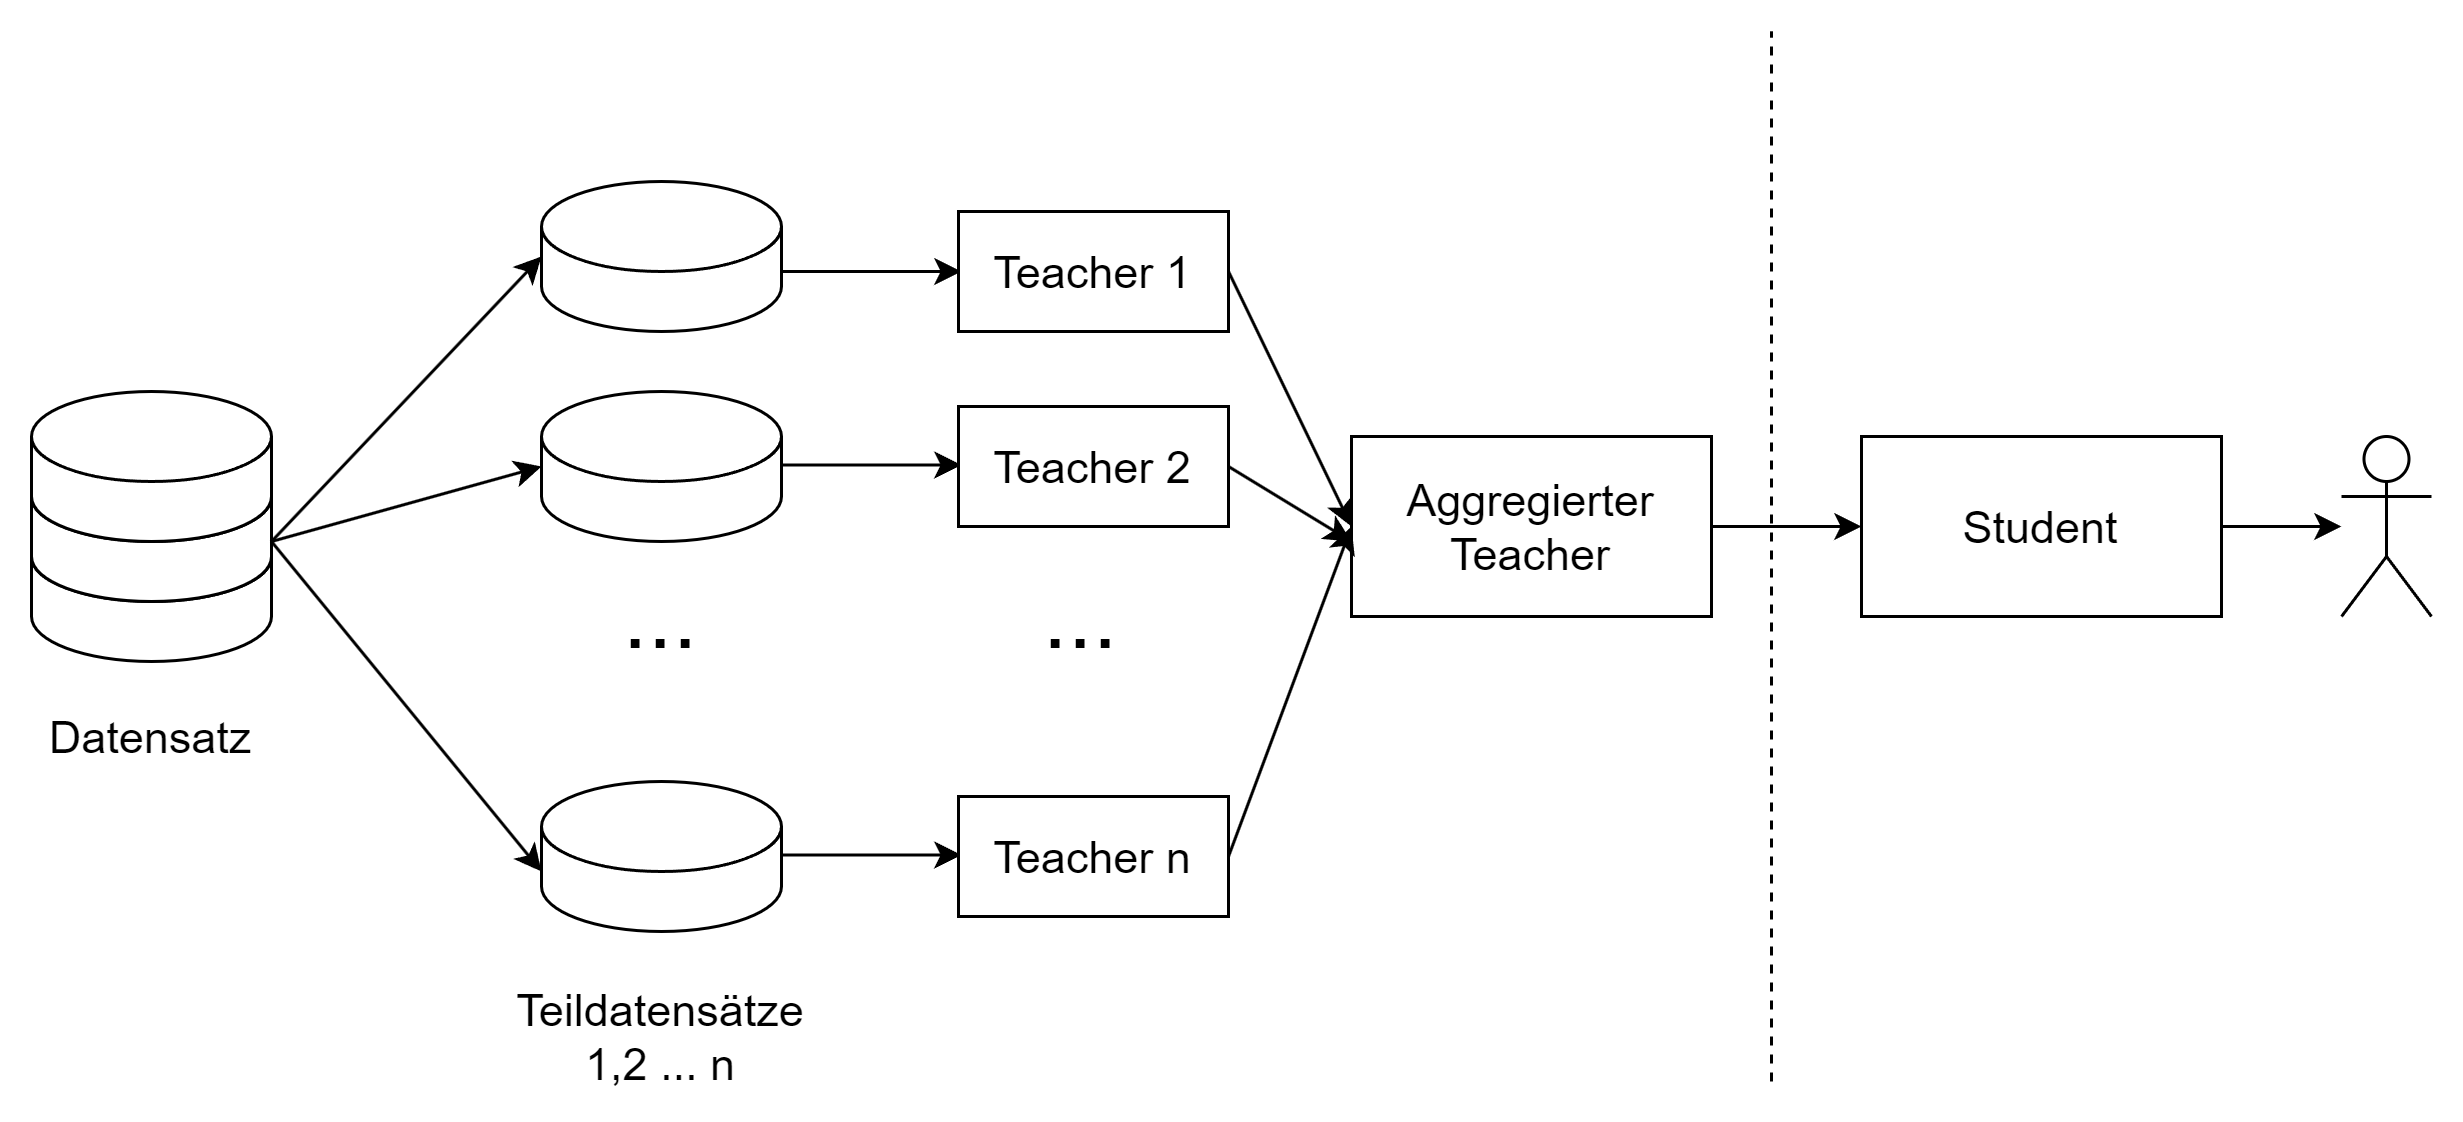
\includegraphics[width=15cm]{figures/pate_basic.png}
    \caption{PATE Architektur nach \cite{P-57}}
    \label{fig:pate_basic}
\end{figure} 

Abbildung \ref{fig:pate_basic} zeigt eine Übersicht der PATE Architektur.
Der Datensatz wird dabei zuerst in verschiedene Teildatensätze aufgeteilt. 
Für jeden dieser Teildatensätze wird anschließend ein sogenanntes Teacher oder Lehrer Modell trainiert.
Wenn das gesamte Modell eine Klassifikation aus 10 unterschiedlichen Klassen ist, dann muss jedes Teacher Modell ebenfalls diese Klassen abbilden.
Hierbei ist es ebenfalls wichtig, dass die Teildatensätze nicht zu klein sind, da ansonsten die Teacher Modelle nicht gut funktionieren würden.
Die Vorhersagen aller Teacher Modelle können aggregiert werden, indem die Vorhersagen der Teacher Modelle addiert werden. 
An dieser Stelle werden die Anzahlen jeder Klasse mittels des Laplace-Mechanismus verrauscht.
Diese Verteilungen können nun an das sogenannte Student oder Schüler Modell weitergegeben werden, um dieses zu trainieren.
Das Student Modell ist auch das einzige, welches für den Nutzer erreichbar ist.
In Abbildung \ref{fig:pate_basic} ist dies der rechte Teil der gestrichelten Linie.
Der linke Teil, die Teacher Modelle sowie die Aggregation dieser, werden für die Vorhersage genutzt, sind aber nicht direkt erreichbar.

Die Autoren untersuchten mehrere Möglichkeiten, das Student Modell zu trainieren.
Die erfolgreichste Methode war ein teilweise beaufsichtigtes (semi-supervised) Lernen, welches auf GANs basiert.
Diese wird folglich PATE-G genannt.
Es können öffentliche, unsensible oder auch ungelabelte Daten zusätzlich genutzt werden.
Teilweise können die ungelabelten Daten mit der Aggregation der Teacher Modelle gelabelt werden, dies ist jedoch nicht für alle Datenpunkte notwendig.
PATE-G nutzt den Student als Diskriminator eines GANs, der eine Klasse für unechte Daten besitzt. 
Anstelle der Klasse für echte Daten, gibt es jedoch Neuronen für jede Klasse des Datensatzes.
Der Generator erzeugt Verteilungen, die den Aggregationen der Teacher Modelle ähnelt.
Das Student Modell, der Diskriminator, soll während des Trainings falsche Verteilungen in die Klasse für unechte Daten einordnen.
Echte, gelabelte Daten (beziehungsweise deren aggregierte Vorhersage) sollen der richtigen Klasse zugeordnet werden, wohingegen echte, ungelabelte Daten irgendeiner beliebigen, echten Klasse zugeordnet werden können.
Abbildung \ref{fig:pate_g} zeigt die bereits beschriebene Trainingsarchitektur von PATE-G.

\begin{figure}[!htb]
    \centering
    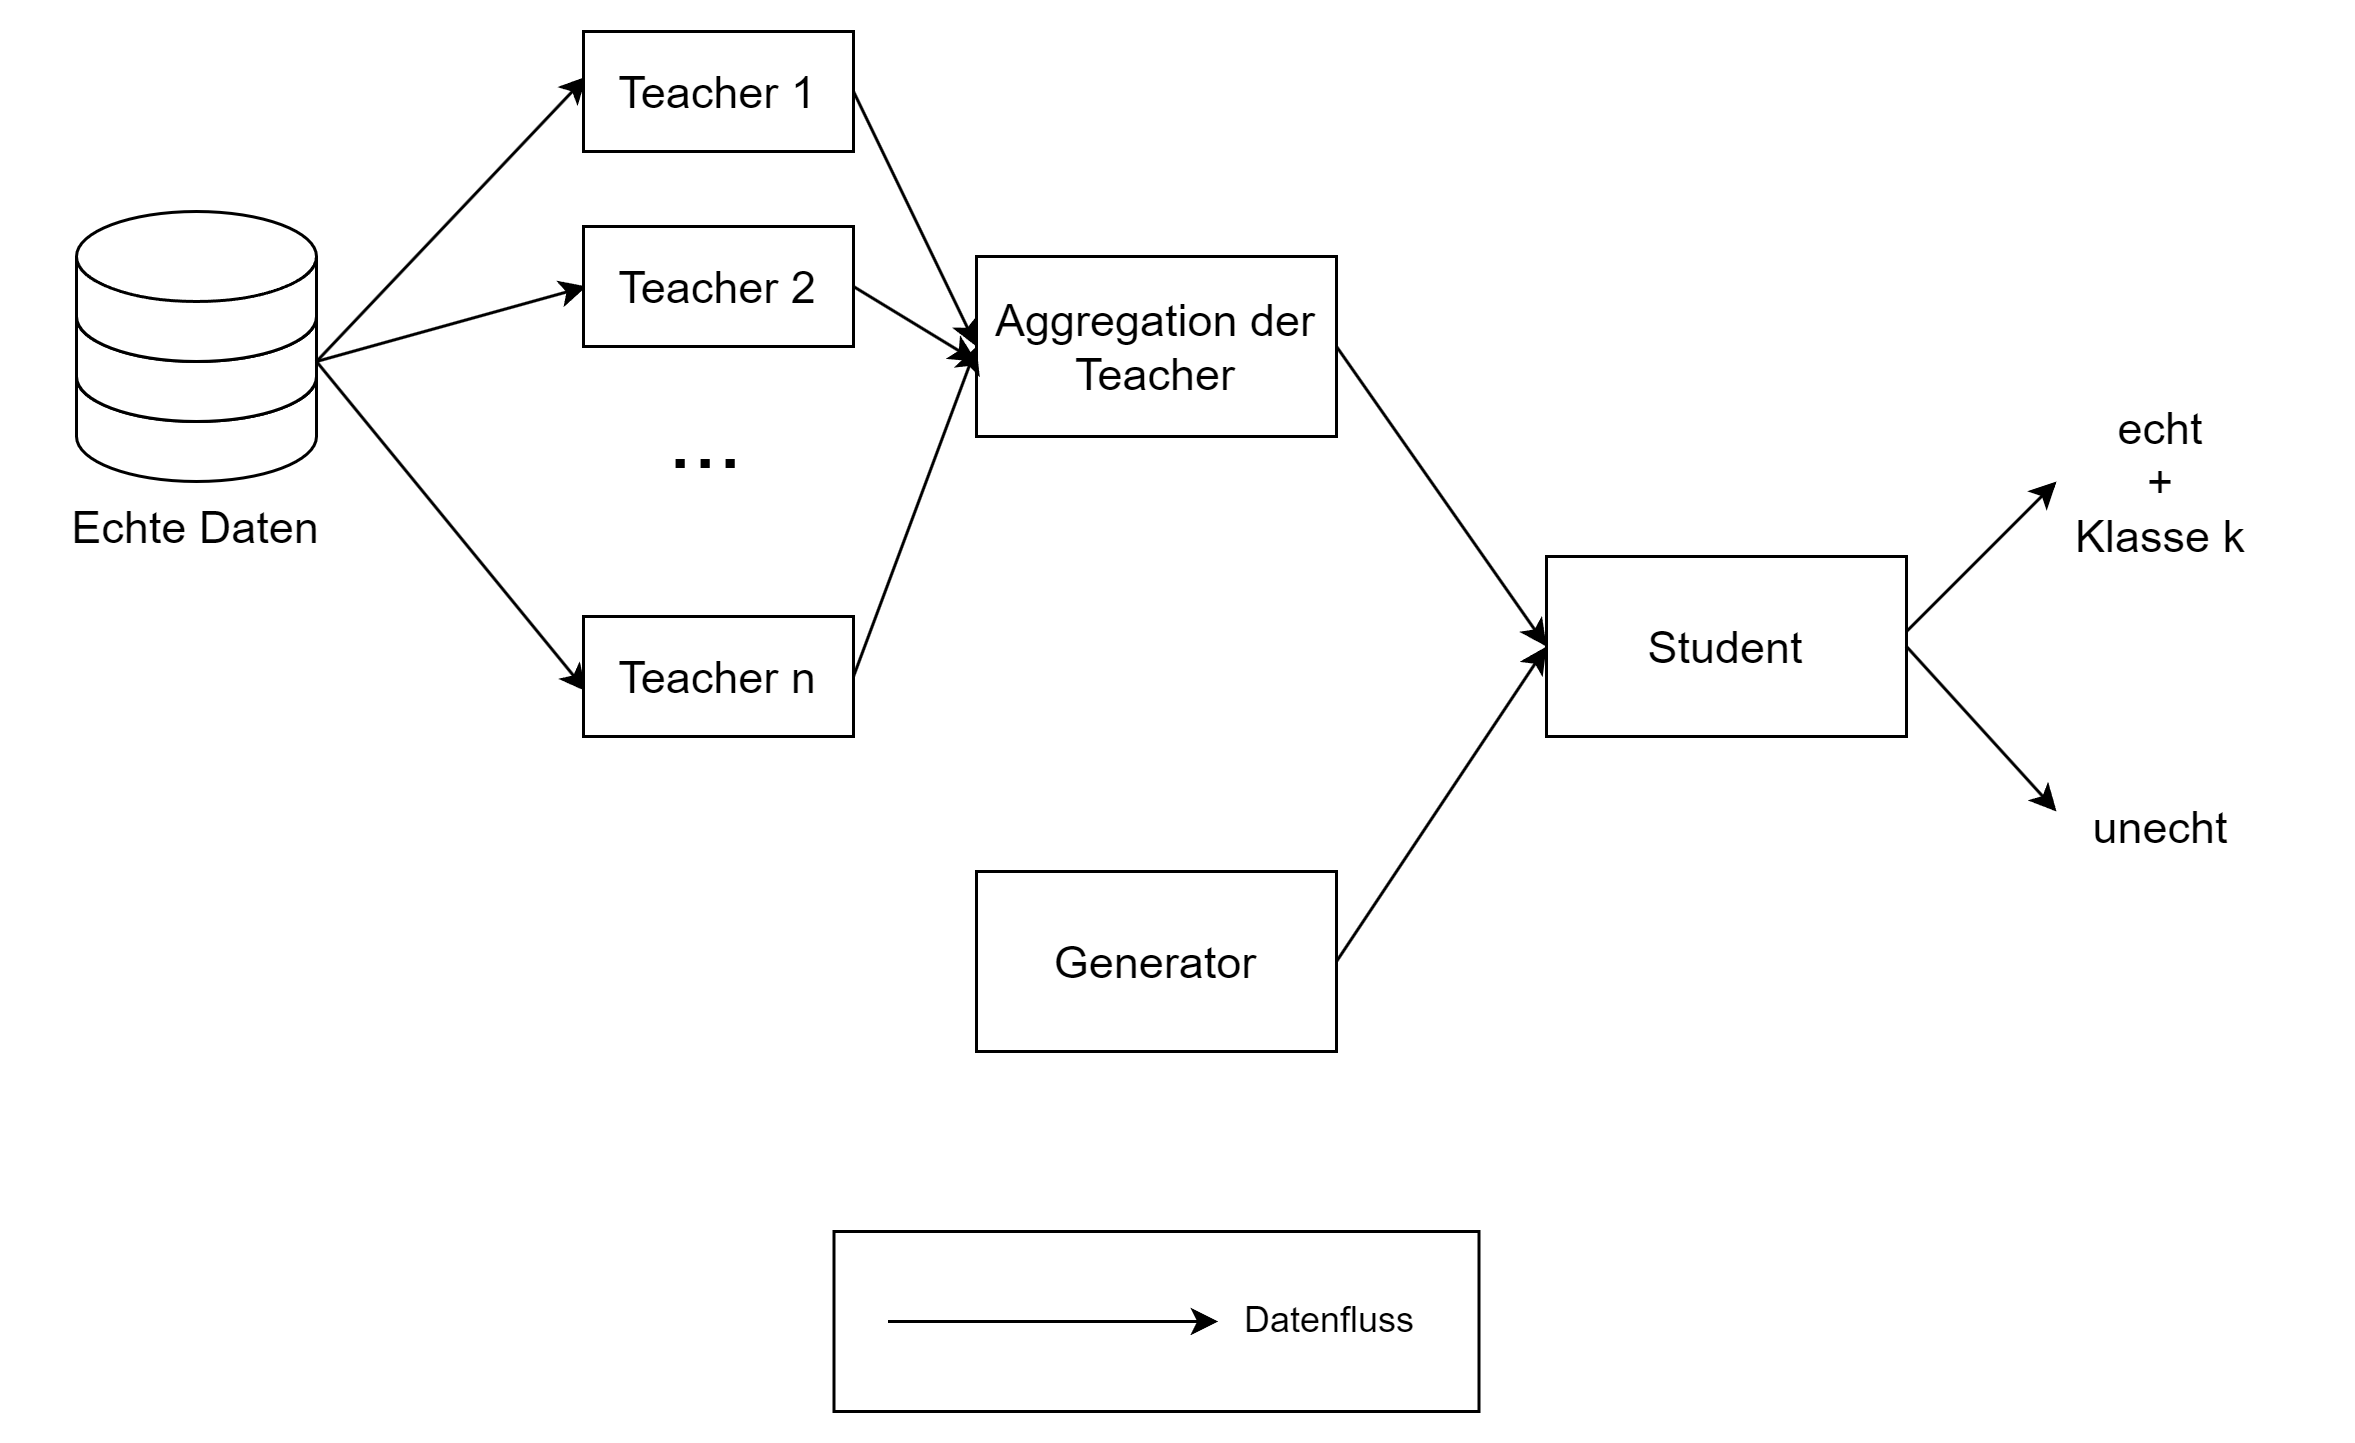
\includegraphics[width=15cm]{figures/pate_g.png}
    \caption{PATE-G}
    \label{fig:pate_g}
\end{figure} 

Die Anzahl der Teacher Modelle beeinflusst die Güte des Modells weniger als die Wahl des Privacy Budgets $\epsilon$.
Umso weniger Teacher vorhanden sind, umso größer sollte $\epsilon$ gewählt werden, damit die Genauigkeit des Modells möglichst groß ist.


